\section{Excercise GettingStartedWithCarRentalCLI}
\subsection*{Analyze the CLI Parameters}
After analyzing the use cases presented in section 3.1 of the goLang tasks in table 4.1, the parameters displayed in figure \ref{fig:car_rental_cli_parameters} are needed.

\begin{figure}[H]
    \centering
    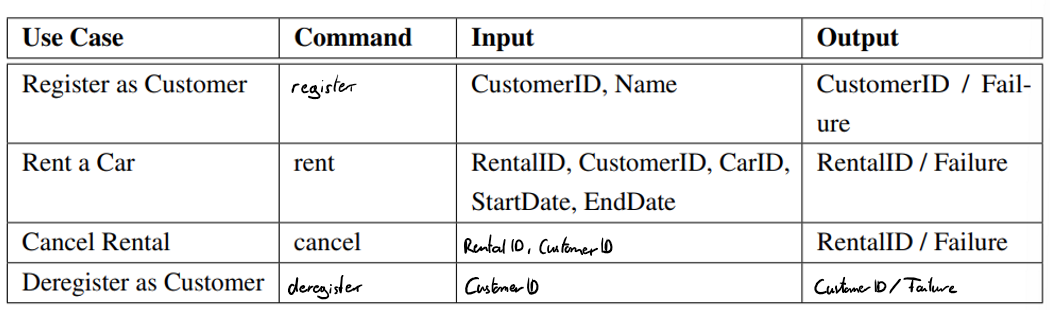
\includegraphics[width=\textwidth]{figures/goLang/carRental/carRental_CLIParameters.png}
    \caption{CLI Parameters}
    \label{fig:car_rental_cli_parameters}
\end{figure}

\subsection*{Describe the Software Architecture}
The given task starts with three different software components:
\begin{itemize}
    \item Presentation Layer: CarRentalCLI
    \item Application Logic Layer: CarRentalOperations
    \item Infrastructure Layer: CarRentalRepository
\end{itemize}
\subsubsection*{Presentation Layer: CarRentalCLI}
This layer consists out of two files: \texttt{CarRentalCli.go} and \texttt{CliActions.go}.
\texttt{CarRentalCli.go} creates a new CLI-object and returns it.
It defines the CLI-commands and their corresponding functions.
It also implements the function to run the CLI, also providing error functions in case of an anomaly.
\texttt{CliActions.go} implements the functions that are called from the CarRentalCli.

\subsubsection*{Application Logic Layer: CarRentalOperations}

